\حصہ{صلیبی ضرب}
اس حصہ میں سمتیات کے ضرب کی دوسری قسم پر غور کیا جائے گا جس کو صلیبی ضرب کہتے ہیں۔ چونکہ صلیبی ضرب کا حاصل سمتی ہوتا ہے لہٰذا اس ضرب کو \اصطلاح{سمتی ضرب}\فرہنگ{ضرب!سمتی}\فرہنگ{سمتی!ضرب}\حاشیہب{vector product}\فرہنگ{vector!product} بھی کہتے ہیں۔

برقیات، مقناطیسیات، صلیبی ضرب، حرکت سیال اور میکانیات مدار میں قوتوں کے اثرات پر غور میں صلیبی ضرب اہم کردار ادا کرتے ہیں۔ آئیں صلیبی ضرب کے خواص پر غور کریں۔ 

\جزوحصہء{دو سمتیات کا صلیبی ضرب}
ہم خلا میں دو غیر صفر سمتیات \عددی{\kvec{A}} اور \عددی{\kvec{B}} سے شروع کرتے ہیں۔ غیر متوازی سمتیات \عددی{\kvec{A}} اور \عددی{\kvec{B}} سطح کو ظاہر کرتے ہیں۔ ہم \اصطلاح{دائیں ہاتھ قاعدہ} سے اس سطح پر عمودی اکائی سمتیہ \عددی{\kvec{n}} منتخب کرتے ہیں۔ یوں سطح میں  \عددی{\kvec{A}} سے \عددی{\kvec{B}} کی جانب دائیں ہاتھ کی انگلیاں، زاویہ \عددی{\theta}  موڑنے سے،  انگوٹھا \عددی{\kvec{n}} کا رخ دے گا (شکل \حوالہ{شکل_سمتیہ_صلیبی_ضرب_مثبت})۔ دائیں ہاتھ کی انگلیاں موڑتے ہوئے زاویہ \عددی{0\le \theta\le \pi} لیا جاتا ہے۔ ہم سمتی ضرب \عددی{\kvec{A}\times\kvec{B}} کی تعریف درج ذیل لیتے ہیں۔

\ابتدا{تعریف} 
\begin{align}\label{مساوات_سمتیہ_تعریف_سمتی_ضرب}
\kvec{A}\times\kvec{B}=(\abs{\kvec{A}}\abs{\kvec{B}}\sin\theta)\kvec{n}
\end{align}
\انتہا{تعریف}
چونکہ سمتیہ \عددی{\kvec{A}\times\kvec{B}} اکائی عمودی سمتیہ \عددی{\kvec{n}} کا غیر سمتی مضرب ہے لہٰذا یہ \عددی{\kvec{A}} اور \عددی{\kvec{B}} دونوں کو عمودی ہو گا۔ سمتیات \عددی{\kvec{A}} اور \عددی{\kvec{B}} کے سمتی ضرب کو عموماً \عددی{\kvec{A}} اور \عددی{\kvec{B}} کا \اصطلاح{صلیبی ضرب}\فرہنگ{صلیبی!ضرب}\فرہنگ{ضرب!صلیبی}\حاشیہب{cross product}\فرہنگ{product!cross} کہتے ہیں۔ صلیبی ضرب کو صلیب کے نشان \عددی{\times} سے ظاہر کیا جاتا ہے اور اسی کی بنا یہ صلیبی ضرب کہلاتا ہے۔
%=========================

\begin{figure}
\centering
\begin{minipage}{0.45\textwidth}
\centering
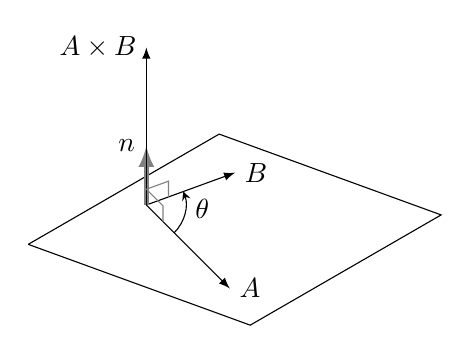
\begin{tikzpicture}
\pgfmathsetmacro{\la}{3}
\pgfmathsetmacro{\aa}{-20}
\pgfmathsetmacro{\lb}{2.8}
\pgfmathsetmacro{\bb}{30}
\draw(0,0)--++(\aa:\la)--++(\bb:\lb)--++(\aa:-\la)--++(\bb:-\lb);
\draw[-latex](1.5,0.5)--++(-45:1.5)coordinate(a)node[right]{$\kvec{A}$};
\draw[-latex](1.5,0.5)--++(20:1.2)coordinate(b)node[right]{$\kvec{B}$};
\draw[-stealth]([shift={(-45:0.5)}]1.5,0.5) arc (-45:20:0.5)node[pos=0.6,right]{$\theta$};
\draw[ultra thick,gray,-latex](1.5,0.5)--++(0,0.75)node[left,black]{$\kvec{n}$};
\draw[-latex](1.5,0.5)--++(0,2)coordinate(n)node[left]{$\kvec{A}\times\kvec{B}$};
\draw[gray](1.5,0.5)++(0,0.2)--++(20:0.3)--++(0,-0.2);
\draw[gray](1.5,0.5)++(0,0.2)--++(-45:0.3)--++(0,-0.2);
\end{tikzpicture}
\caption{صلیبی ضرب \عددی{\kvec{A}\times\kvec{B}}}
\label{شکل_سمتیہ_صلیبی_ضرب_مثبت}
\end{minipage}\hfill
\begin{minipage}{0.45\textwidth}
\centering
\begin{tikzpicture}
\pgfmathsetmacro{\la}{3}
\pgfmathsetmacro{\aa}{-20}
\pgfmathsetmacro{\lb}{2.8}
\pgfmathsetmacro{\bb}{30}
\draw[name path=pl](0,0)--++(\aa:\la)--++(\bb:\lb)--++(\aa:-\la)--++(\bb:-\lb);
\draw[-latex](1.5,0.5)--++(-45:1.5)coordinate(a)node[right]{$\kvec{A}$};
\draw[-latex](1.5,0.5)--++(20:1.2)coordinate(b)node[right]{$\kvec{B}$};
\draw[-stealth]([shift={(20:0.5)}]1.5,0.5) arc (20:-45:0.5)node[pos=0.4,right]{$\theta$};
\path[name path=cr](1.5,0.5)--++(0,-2)coordinate(ktip);
\draw[ultra thick,gray,-latex](1.5,0.5)--++(0,-0.75)node[left,black]{$\kvec{n}$};
\draw[thick,dashed,name intersections={of=cr and pl}](1.5,0.5)--(intersection-1);
\draw[-latex](intersection-1)--(ktip)coordinate(n)node[left]{$\kvec{B}\times\kvec{A}$};
\draw[gray](1.5,0.5)++(0,-0.2)--++(20:0.3)--++(0,0.2);
\draw[gray](1.5,0.5)++(0,-0.2)--++(-45:0.3)--++(0,0.2);
\end{tikzpicture}
\caption{صلیبی ضرب \عددی{\kvec{B}\times\kvec{A}}}
\label{شکل_سمتیہ_صلیبی_ضرب_منفی}
\end{minipage}
\end{figure}

چونکہ \عددی{0} اور \عددی{\pi} کے سائن صفر ہوتے ہیں لہٰذا ہم مساوات \حوالہ{مساوات_سمتیہ_تعریف_سمتی_ضرب} میں دو غیر صفر متوازی سمتیات کے صلیبی ضرب کی تعریف \عددی{\kvec{0}} لیں گے۔

اگر \عددی{\kvec{A}} یا \عددی{\kvec{B}} صفر ہو تب ہم \عددی{\kvec{A}\times\kvec{B}} کی قیمت صفر لیں گے۔ یوں دو سمتیات \عددی{\kvec{A}} اور \عددی{\kvec{B}} کا صلیبی ضرب صرف اور صرف اس صورت صفر ہو گا جب \عددی{\kvec{A}} اور \عددی{\kvec{B}} متوازی ہوں یا ان میں سے ایک یا دونوں صفر ہوں۔ اس طرح غیر صفر سمتیات کا صلیبی ضرب صرف اور صرف اس صورت صفر ہو گا جب یہ متوازی ہوں۔

\جزوحصہء{\عددی{\kvec{A}\times\kvec{B}}  بالمقابل \عددی{\kvec{B}\times\kvec{A}}}
غیر صفر سمتی ضرب میں سمتیات کی ترتیب بدلنے سے حاصل ضرب کی سمت الٹ ہوتی ہے۔ اگر ہم سمتیہ \عددی{\kvec{B}} سے \عددی{\kvec{A}} کی جانب دائیں ہاتھ کی انگلیوں کو، زاویہ \عددی{\theta}  موڑیں، تب ہمارا انگوٹھا پہلے رخ کا مخالف رخ دے گا (یہاں پہلے رخ سے مراد \عددی{\kvec{A}\times\kvec{B}} کے حصول میں انگوٹھے کا رخ ہے)۔ دائیں ہاتھ کی انگلیاں موڑتے ہوئے زاویہ \عددی{0\le\theta\le\pi} لیا جاتا ہے۔  شکل \حوالہ{شکل_سمتیہ_صلیبی_ضرب_منفی} میں ان نتائج کو دکھایا گیا ہے۔ یوں تمام سمتیات \عددی{\kvec{A}} اور \عددی{\kvec{B}} کے لئے درج ذیل ہو گا۔
\begin{align}
\kvec{B}\times\kvec{A}=-(\kvec{A}\times\kvec{B})
\end{align}
ضرب نقطہ کے برعکس صلیبی ضرب \اصطلاح{نا قابل تبادل}\فرہنگ{قابل تبادل!نا}\حاشیہب{non commutative}\فرہنگ{commutative!non} ہے۔

صلیبی ضرب کی تعریف \عددی{\ai}، \عددی{\aj} اور \عددی{\ak} کی جوڑیوں پر لاگو کرتے ہوئے درج ذیل نتائج حاصل ہوتے ہیں جنہیں دکھائے گئے دائرے سے با آسانی یاد رکھا جا سکتا ہے۔

\begin{minipage}{0.25\textwidth}
\centering
\begin{tikzpicture}
\draw[-stealth]([shift={(-90+20:1)}]0,0) arc (-90+20:30:1)node[pos=0,fill=white]{$\ai$};
\draw[-stealth]([shift={(30+20:1)}]0,0) arc (30+20:150:1)node[pos=0,fill=white]{$\aj$};
\draw[-stealth]([shift={(150+20:1)}]0,0) arc (150+20:270:1)node[pos=0,fill=white]{$\ak$};
\end{tikzpicture}
\end{minipage}\hfill
\begin{minipage}{0.65\textwidth}
\centering
\begin{gather}
\begin{aligned}
\ai\times\aj&=-(\aj\times\ai)=\ak\\
\aj\times\ak&=-(\ak\times\aj)=\ai\\
\ak\times\ai&=-(\ai\times\ak)-\aj
\end{aligned}
\end{gather}
\end{minipage}

اکائی سمتیات کے ہم صلیبی ضرب صفر ہوں گے:
\begin{align*}
\kvec{\ai}\times\kvec{i}&=(\abs{\ai}\abs{\ai}\sin0^{\circ})\kvec{n}=((1)(1)(0))\kvec{n}=0\\
\kvec{\aj}\times\kvec{\aj}&=(\abs{\aj}\abs{\aj}\sin0^{\circ})\kvec{n}=((1)(1)(0))\kvec{n}=0\\
\kvec{\ak}\times\kvec{\ak}&=(\abs{\ak}\abs{\ak}\sin0^{\circ})\kvec{n}=((1)(1)(0))\kvec{n}=0
\end{align*}

\جزوحصہء{صلیبی ضرب \عددی{\kvec{A}\times\kvec{B}} متوازی الاضلاع کا رقبہ ہو گا}
چونکہ \عددی{\kvec{n}} اکائی سمتیہ ہے لہٰذا \عددی{\kvec{A}\times\kvec{B}} کی مقدار
\begin{align}\label{مساوات_سمتیہ_صلیبی_ضرب_کی_مقدار}
\abs{\kvec{A}\times\kvec{B}}=\abs{\kvec{A}}\abs{\kvec{B}}\abs{\sin\theta}\abs{\kvec{n}}=\abs{\kvec{A}}\abs{\kvec{B}}\sin\theta
\end{align}
ہو گی جو اس متوازی الاضلاع کا رقبہ ہے جس کے ضلع \عددی{\kvec{A}} اور \عددی{\kvec{B}} ہیں۔ اس متوازی الاضلاع کا قاعدہ \عددی{\abs{\kvec{A}}} جبکہ اس کا قد \عددی{\abs{\kvec{B}\sin\theta}} ہے (شکل \حوالہ{شکل_سمتیہ_رقبہ_متوازی_الاضلاع})۔
\begin{figure}
\centering
\begin{tikzpicture}
\draw[-latex](0,0)--(3,0)node[pos=0.75,below]{$\kvec{A}$};
\draw[-latex](0,0)--++(30:2)coordinate(kt)node[pos=0.5,above left]{$\kvec{B}$};
\draw([shift={(0:0.5)}]0,0) arc (0:30:0.5)node[pos=0.7,right]{$\theta$};
\draw[](0,0)++(3,0)--++(30:2);
\draw[](0,0)++(30:2)--++(3,0);
\draw[dashed](kt)--($(0,0)!(kt)!(3,0)$)node[pos=0.5,right]{$\abs{\kvec{B}}\abs{\sin\theta}$};
\end{tikzpicture}
\caption{متوازی الاضلاع کا رقبہ اس کے قاعدہ ضرب قد کے برابر ہوتا ہے۔}
\label{شکل_سمتیہ_رقبہ_متوازی_الاضلاع}
\end{figure}

\جزوحصہء{قوت مروڑ}
نقطہ \عددی{ N} پر چول کے ساتھ سلاخ  کا ایک سر منسلک ہے جس کے دوسرے سے پر قوت \عددی{\kvec{F}} عمل کرتی ہے۔ چول سے سلاخ کے دوسرے سر تک ہٹاو کو سمتیہ \عددی{\kvec{r}} ظاہر کرتا ہے (شکل \حوالہ{شکل_سمتیہ_قوت_مروڑ_تعریف})۔ قوت مروڑ کی مقدار سے مراد  ہم \عددی{\kvec{r}} کی لمبائی ضرب قوت کا وہ حصہ جو \عددی{\kvec{r}} کو عمودی ہے، لیتے ہیں۔ علامتی طور پر ہم قوت مروڑ سمتیہ کی مقدار کو
\begin{align*}
\text{\RL{قوت مروڑ سمتیہ کی مقدار}}=\abs{\kvec{r}}\abs{\kvec{F}}\sin\theta
\end{align*}
یا \عددی{\abs{\kvec{r}\times\kvec{F}}} لکھ سکتے ہیں۔ ہم دائیں ہاتھ قاعدہ سے حاصل اکائی سمتیہ \عددی{\kvec{n}} استعمال کرتے ہوئے قوت مروڑ سمتیہ کو درج ذیل لکھ سکتے ہیں۔
\begin{align*}
\text{\RL{قوت مروڑ سمتیہ}}=(\abs{\kvec{r}}\abs{\kvec{F}}\sin\theta)\kvec{n}=\kvec{r}\times\kvec{F}
\end{align*}
یاد رہے کہ  (غیر صفر سمتیات کی صورت میں) \عددی{\kvec{A}\times\kvec{B}} تب \عددی{\kvec{0}} ہوتا ہے جب \عددی{\kvec{A}} اور \عددی{\kvec{B}} متوازی ہوں۔ قوت مروڑ کی تعریف عین اس حقیقت کے مطابق ہے۔ یوں اگر قوت عین سلاخ کے متوازی عمل کرے تب حاصل قوت مروڑ صفر ہو گا۔ 
\begin{figure}
\centering
\begin{tikzpicture}
\pgfmathsetmacro{\kx}{1.75*cos(60)}
\draw[-latex](0,0)node[circ]{}node[below]{$N$}--(2,0)node[pos=0.5,above]{$\kvec{r}$};
\draw[-latex](2,0)--++(-60:1.75)coordinate(kt)node[pos=0.5,right]{$\kvec{F}$};
\draw[dashed](2,0)--++(1,0);
\draw([shift={(0:0.3)}]2,0) arc (0:-60:0.3)node[pos=0.7,right]{$\theta$}; 
\draw[dashed](kt)--++(-\kx,0)coordinate(kb);
\draw[-latex](2,0)--(kb)node[pos=0.75,left]{$\abs{\kvec{F}}\sin\theta$};
\RightAngle{(2,0)}{(kb)}{(kt)}
\end{tikzpicture}
\caption{قوت مروڑ۔}
\label{شکل_سمتیہ_قوت_مروڑ_تعریف}
\end{figure}

%======================
\ابتدا{مثال}\شناخت{مثال_سمتیہ_قوت_مروڑ}
قوت مروڑ کی مقدار شکل \حوالہ{شکل_مثال_سمتیہ_قوت_مروڑ} میں درج ذیل ہو گی۔
\begin{align*}
\abs{\krightharpoonup{NQ}\times \kvec{F}}&=\abs{\krightharpoonup{NQ}}\abs{\kvec{F}}\sin 70^{\circ}&&\text{\RL{مساوات \حوالہ{مساوات_سمتیہ_صلیبی_ضرب_کی_مقدار}}}\\
&\approx (3)(20)(0.94)\\
&\approx \SI{56.4}{\newton\meter}
\end{align*}
\انتہا{مثال}
%===============
\begin{figure}
\centering
\begin{tikzpicture}
\pgfmathsetmacro{\kx}{1.75*cos(60)}
\draw[thick](0,0)node[circ]{}node[below]{$N$}--(2,0)node[right]{$Q$}node[pos=0.5,above]{$\SI{3}{\meter}$};
\draw[latex-](2,0)--++(-100:1.75)coordinate(kt)node[pos=0.5,right]{$\SI{20}{\newton}$};
\draw([shift={(180:0.3)}]2,0) arc (180:260:0.3)node[pos=0.7,left]{$70^{\circ}$}; 
\end{tikzpicture}
\caption{قوت مروڑ (مثال \حوالہ{مثال_سمتیہ_قوت_مروڑ})۔}
\label{شکل_مثال_سمتیہ_قوت_مروڑ}
\end{figure}

\جزوحصہء{قوانین تلازم اور تقسیم}
صلیبی ضرب عام طور غیر تلازمی ہو گا چونکہ \عددی{(\kvec{A}\times\kvec{B})\times\kvec{C}} سمتیات \عددی{\kvec{A}} اور \عددی{\kvec{B}} کے مستوی  میں پایا جاتا ہے جبکہ \عددی{\kvec{A}\times(\kvec{B}\times\kvec{C})} سمتیات  \عددی{\kvec{B}} اور \عددی{\kvec{C}} کے مستوی  میں پایا جاتا ہے۔ اس کے باوجود درج ذیل قواعد مطمئن ہوتے ہیں۔
\begin{align}
(r\kvec{A})\times (s\kvec{B})&=(rs)(\kvec{A}\times\kvec{B})&&\text{\RL{غیر سمتی قاعدہ تقسیم}}\label{مساوات_سمتیہ_غیر_سمتی_قاعدہ_تقسیم}\\
\kvec{A}\times (\kvec{B}+\kvec{C})&=\kvec{A}\times\kvec{B}+\kvec{A}\times\kvec{C}&&\text{\RL{سمتی قاعدہ تقسیم}}\label{مساوات_سمتیہ_سمتی_قاعدہ_تقسیم_الف}\\
(\kvec{B}+\kvec{C})\times \kvec{A}&=\kvec{B}\times \kvec{A}+\kvec{C}\times\kvec{A}&&\text{\RL{سمتی قاعدہ تقسیم}}\label{مساوات_سمتیہ_سمتی_قاعدہ_تقسیم_ب}
\end{align}

مساوات \حوالہ{مساوات_سمتیہ_غیر_سمتی_قاعدہ_تقسیم} کی ایک مخصوص صورت درج ذیل ہے۔
\begin{align}\label{مساوات_سمتیہ_غیر_سمتی_قاعدہ_تقسیم_مخصوص}
(-\kvec{A})\times \kvec{B}=\kvec{A}\times(-\kvec{B})=-(\kvec{A}\times\kvec{B})
\end{align}

غیر سمتی قاعدہ تقسیم  ثابت کرنے کی خاطر مساوات \حوالہ{مساوات_سمتیہ_غیر_سمتی_قاعدہ_تقسیم} کے دونوں اطراف پر مساوات \حوالہ{مساوات_سمتیہ_تعریف_سمتی_ضرب} عائد کر کے نتائج کا موازنہ کریں۔ سمتی قاعدہ تقسیم مساوات \حوالہ{مساوات_سمتیہ_سمتی_قاعدہ_تقسیم_الف} کو ثابت کرنا اتنا آسان نہیں ہے۔ ہم اس کی حقیقت کو یہاں تسلیم کرتے ہیں۔ اس کا ثبوت ضمیمہ \حوالہ{ضمیمہ_ز} میں پیش کیا گیا ہے۔ مساوات \حوالہ{مساوات_سمتیہ_سمتی_قاعدہ_تقسیم_ب} کو مساوات \حوالہ{مساوات_سمتیہ_سمتی_قاعدہ_تقسیم_الف} سے اخذ کیا جا سکتا ہے۔ مساوات \حوالہ{مساوات_سمتیہ_سمتی_قاعدہ_تقسیم_الف} کے دونوں اطراف کو \عددی{-1} سے ضرب کر کے حاصل اجزاء کے مقام تبدیل کریں۔

\جزوحصہء{\عددی{\kvec{A}\times\kvec{B}} کا کلیہ بذریعہ مقطع}
ہم \عددی{\kvec{A}\times \kvec{B}} کا حساب  کارتیسی محددی نظام میں \عددی{\kvec{A}} اور \عددی{\kvec{B}} سے کرنا چاہتے ہیں۔ ہم درج ذیل فرض کرتے ہیں۔
\begin{align*}
\kvec{A}=a_1\ai+a_2\aj+a_3\ak,\quad \kvec{B}=b_1\ai+b_2\aj+a_3\ak
\end{align*}
قواعد تقسیم اور \عددی{\ai}، \عددی{\aj} اور \عددی{\ak} کے قواعد ضرب سے درج ذیل حاصل ہو گا۔
\begin{align*}
\kvec{A}\times\kvec{B}&=(a_1\ai+a_2\aj+a_3\ak)\times(b_1\ai+b_2\aj+a_3\ak)\\
&=a_1b_1\ai\times\ai+a_1b_2\ai\times\aj+a_1b_3\ai\times\ak\\
&\phantom{=}+a_2b_1\aj\times\ai+a_2b_2\aj\times\aj+a_2b_3\aj\times\ak\\
&\phantom{=}+a_3b_1\ak\times\ai+a_3b_2\ak\times\aj+a_3b_3\ak\times\ak\\
&=(a_2b_3-a_3b_2)\ai-(a_1b_3-a_3b_1)\aj+(a_1b_2-a_2b_1)\ak
\end{align*}  

مذکورہ بالا مساوات کا آخری حصہ قالب
\begin{align*}
\begin{vmatrix}
\ai&\aj&\ak\\
a_1&a_2&a_3\\
b_1&b_2&b_3
\end{vmatrix}
\end{align*}  
 کو کھول کر ملتا ہے۔

یوں اگر سمتیات \عددی{\kvec{A}=a_1\ai+a_2\aj+a_3\ak} اور \عددی{\kvec{B}=b_1\ai+b_2\aj+b_3\ak} ہوں تب درج ذیل ہو گا۔
\begin{align}
\kvec{A}\times\kvec{B}=
\begin{vmatrix}
\ai&\aj&\ak\\
a_1&a_2&a_3\\
b_1&b_2&b_3
\end{vmatrix}
\end{align}

\ابتدا{مثال}
\begin{align*}
\begin{vmatrix}a&b\\c&d  \end{vmatrix}=ad-bc
\end{align*}
\انتہا{مثال}
%====================
\ابتدا{مثال}
\begin{align*}
\begin{vmatrix} 2&1\\-4&3 \end{vmatrix}=(2)(3)-(1)(-4)=6+4=10
\end{align*}
\انتہا{مثال}
%=================
\ابتدا{مثال}
\begin{align*}
\begin{vmatrix} a_1&a_2&a_3\\ b_1&b_2&b_3\\c_1&c_2&c_3 \end{vmatrix}=
a_1\begin{vmatrix} b_2&b_3\\ c_2&c_3\end{vmatrix}-a_2\begin{vmatrix} b_1&b_3\\c_1&c_3 \end{vmatrix}+a_3\begin{vmatrix} b_1&b_2\\c_1&c_2 \end{vmatrix}
\end{align*}
\انتہا{مثال}
%=======================
\ابتدا{مثال}
\begin{align*}
\begin{vmatrix} -5&3&1\\2&1&1\\-4&3&1\end{vmatrix}&=
(-5)\begin{vmatrix} 1&1\\3&1\end{vmatrix}-(3)\begin{vmatrix}2 &1\\ -4&1\end{vmatrix}+(1)\begin{vmatrix} 2&1\\-4&3 \end{vmatrix}\\
&=-5(1-3)-3(2+4)+1(6+4)=10-18+10=2
\end{align*}
\انتہا{مثال}
%==========================
\ابتدا{مثال}
صلیبی ضرب \عددی{\kvec{A}\times\kvec{B}} اور \عددی{\kvec{B}\times\kvec{A}} درج ذیل سمتیات کے لئے حاصل کریں۔
\begin{align*}
\kvec{A}=2\ai+\aj+\ak,\quad \kvec{B}=-4\ai+3\aj+\ak
\end{align*}
حل:
\begin{align*}
\kvec{A}\times\kvec{B}&=
\begin{vmatrix}
\ai&\aj&\ak\\
2&1&1\\
-4&3&1
\end{vmatrix}=
\begin{vmatrix} 1&1\\ 3&1 \end{vmatrix}\ai-\begin{vmatrix}2&1\\-4&1  \end{vmatrix}\aj+\begin{vmatrix}2&1\\-4&3  \end{vmatrix}\ak\\
&=-2\ai-6\aj+10\ak\\
\kvec{B}\times\kvec{A}&=-(\kvec{A}\times\kvec{B})=2\ai+6\aj-10\ak
\end{align*}
\انتہا{مثال}
%=============
\ابتدا{مثال}\شناخت{مثال_سمتیہ_مستوی_کو_عمودی}
ایک مستوی پر نقاط \عددی{P(1,-1,0)}، \عددی{Q(2,1,-1)} اور \عددی{R(-1,1,2)} پائے جاتے ہیں۔ اس سطح کو عمودی سمتیہ تلاش کریں۔

حل:\quad
سمتیات \عددی{\krightharpoonup{PQ}} اور \عددی{\krightharpoonup{PR}} اس سطح میں پائے جائیں گے۔ چونکہ سمتیہ \عددی{\krightharpoonup{PQ}\times\krightharpoonup{PR}} ان دونوں سمتیات کو عمودی ہے لہٰذا یہ مستوی کو بھی عمودی ہو گا۔ اجزاء کی صورت میں درج ذیل ہو گا۔
\begin{align*}
\krightharpoonup{PQ}&=(2-1)\ai+(1+1)\aj+(-1-0)\ak=\ai+2\aj-\ak\\
\krightharpoonup{PR}&=(-1-1)\ai+(1+1)\aj+(2-0)\ak=-2\ai+2\aj+2\ak\\
\krightharpoonup{PQ}\times\krightharpoonup{PR}&=
\begin{vmatrix}
\ai&\aj&\ak\\
1&2&-1\\
-2&2&2
\end{vmatrix}=
\begin{vmatrix}2&-1\\2&2  \end{vmatrix}\ai-\begin{vmatrix} 1&-1\\-2&2 \end{vmatrix}\aj+\begin{vmatrix}1&2\\-2&2  \end{vmatrix}\ak\\
&=6\ai+6\ak
\end{align*}
\انتہا{مثال}
%==========
\ابتدا{مثال}
ایک مثلث کے راس \عددی{P(1,-1,0)}، \عددی{Q(2,1,-1)} اور \عددی{R(-1,1,2)} ہیں۔ اس مثلث کا رقبہ معلوم کریں۔

حل:\quad
سمتیات \عددی{\krightharpoonup{PQ}} اور \عددی{\krightharpoonup{PR}} جس متوازی الاضلاع کے ضلع ہوں اس کا رقبہ درج ذیل ہو گا۔
\begin{align*}
\abs{\krightharpoonup{PQ}\times\krightharpoonup{PR}}&=\abs{6\ai+6\ak}&&\text{\RL{مثال \حوالہ{مثال_سمتیہ_مستوی_کو_عمودی}}}\\
&=\sqrt{(6)^2+(6)^2}=6\sqrt{2}
\end{align*}
مثلث کا رقبہ اس کا نصف \عددی{3\sqrt{2}} ہو گا۔
\انتہا{مثال}
%============
\ابتدا{مثال}
سطح \عددی{P(1,-1,0)}، \عددی{Q(2,1,-1)} اور \عددی{R(-1,1,2)} کا عمودی اکائی سمتیہ \عددی{\kvec{n}} دریافت کریں۔

حل:\quad
چونکہ \عددی{\krightharpoonup{PQ}\times \krightharpoonup{PR}} مستوی کو عمودی ہے لہٰذا \عددی{\kvec{n}} کا رخ یہی سمتیہ دے گا۔ہم اس سمتیہ کو اس کی مقدار سے تقسیم کر کے عمودی اکائی سمتیہ معلوم کرتے ہیں۔
\begin{align*}
\kvec{n}&=\frac{\krightharpoonup{PQ}\times \krightharpoonup{PR}}{\abs{\krightharpoonup{PQ}\times \krightharpoonup{PR}}}=\frac{6\ai+6\ak}{6\sqrt{2}}=\frac{1}{\sqrt{2}}\ai+\frac{1}{\sqrt{2}}\ak
\end{align*}
چونکہ سطح کے دو آپس میں مخالف رخ عمودی سمتیات پائے جاتے ہیں لہٰذا اس سطح کا دوسرا عمودی اکائی سمتیہ \عددی{-\tfrac{1}{\sqrt{2}}\ai-\tfrac{1}{\sqrt{2}}\ak} ہو گا۔ 
\انتہا{مثال}
%================

\جزوحصہء{غیر سمتی سہ ضرب}
ضرب \عددی{(\kvec{A}\times\kvec{B})\cdot \kvec{C}} کو \عددی{\kvec{A}}، \عددی{\kvec{B}} اور \عددی{\kvec{C}} کا غیر سمتی سہ ضرب کہتے ہیں جہاں سمتیات کی ترتیب یہی ہے۔ آپ دیکھ سکتے ہیں (شکل \حوالہ{شکل_سمتیہ_حجم_مستطیلی_متوازی_السطوح}) کہ غیر سمتی سہ ضرب کی مطلق قیمت
\begin{align*}
\abs{(\kvec{A}\times\kvec{B})\cdot\kvec{C}}=\abs{\kvec{A}\times\kvec{B}}\abs{\kvec{C}}\abs{\cos\theta}
\end{align*}
 اس مستطیلی متوازی السطوح کا حجم دیتی ہے جس کے اضلاع \عددی{\kvec{A}}، \عددی{\kvec{B}} اور \عددی{\kvec{C}} ہوں۔ مستطیلی متوازی السطوح کا حجم اس کے  قاعدہ کا رقبہ \عددی{\abs{\kvec{A}\times \kvec{B}}} اور اس کے قد \عددی{\abs{\kvec{C}}\abs{\cos\theta}} کا حاصل ضرب نقطہ 
\begin{align*}
\text{حجم}&=(\text{\RL{رقبہ قاعدہ}})\cdot(\text{قد})\\
&=\abs{\kvec{A}\times\kvec{B}}\cdot\abs{\kvec{C}}\abs{\cos\theta}\\
&=\abs{(\kvec{A}\times\kvec{B})\cdot\kvec{C}}
\end{align*}
 ہو گا۔
\begin{figure}
\centering
\begin{tikzpicture}
\pgfmathsetmacro{\a}{3}
\pgfmathsetmacro{\b}{1.5}
\pgfmathsetmacro{\c}{2}
\pgfmathsetmacro{\aa}{0}
\pgfmathsetmacro{\bb}{30}
\pgfmathsetmacro{\cc}{60}
\draw[fill=llgray](0,0)--++(\aa:\a)--++(\bb:\b)--++(\aa:-\a)--(0,0);
\draw[-latex](0,0)coordinate(O)--++(\aa:\a)coordinate(a)node[pos=0.5,below]{$\kvec{A}$};
\draw[-latex](0,0)--++(\bb:\b)coordinate(b)node[pos=0.9,left,yshift=1ex]{$\kvec{B}$};
\draw[-latex](0,0)--++(\cc:\c)coordinate(c)node[pos=0.75,left]{$\kvec{C}$};
\draw(a)--++(\cc:\c)coordinate(ac)--(c);
\draw(a)--++(\bb:\b)coordinate(ab)--(b);
\draw(c)--++(\bb:\b)coordinate(bc)--++(\aa:\a)coordinate(abc)--(ac);
\draw(abc)--(ab);
\draw(bc)--(b);
\draw[-latex](0,0)--++(0,3)node[left]{$\kvec{A}\times\kvec{B}$};
\draw[dashed](c)--($(0,0)!(c)!(0,3)$)coordinate(h);
\draw[stealth-stealth]($(h)+(-0.3,0)$)--(-0.3,0)node[pos=0.5,left]{قد$=\abs{\kvec{C}}\abs{\cos\theta}$};
\draw([shift={(\cc:0.5)}]0,0) arc (\cc:90:0.5)node[pos=0.4,above]{$\theta$};
\draw($(h)+(-0.2,0)$)--++(-0.2,0);
\draw(-0.2,0)--++(-0.2,0);
\draw($(a)!0.6!(ab)$)++(-0.5,0)node[pin=-30:{\RL{رقبہ قاعدہ }$=\abs{\kvec{A}\times\kvec{B}}$}]{};
\end{tikzpicture}
\caption{مستطیلی متوازی السطوح کا حجم اس کے قاعدہ کا رقبہ ضرب قد کے برابر ہو گا۔}
\label{شکل_سمتیہ_حجم_مستطیلی_متوازی_السطوح}
\end{figure} 

سمتیات \عددی{\kvec{A}} اور \عددی{\kvec{B}} کی سطح کو شکل \حوالہ{شکل_سمتیہ_حجم_مستطیلی_متوازی_السطوح} میں قاعدہ دکھایا گیا ہے۔ ہم
سمتیات \عددی{\kvec{B}} اور \عددی{\kvec{C}} کی سطح یا  سمتیات \عددی{\kvec{C}} اور \عددی{\kvec{A}} کی سطح کو قاعدہ لے کر بھی حجم تلاش کر سکتے ہیں۔ چونکہ حجم اٹل قیمت ہے لہٰذا درج ذیل حاصل ہو گا۔
\begin{align}\label{مساوات_سمتیہ_حجم_کی_مساوات}
(\kvec{A}\times\kvec{B})\cdot\kvec{C}=(\kvec{B}\times\kvec{C})\cdot\kvec{A}=(\kvec{C}\times\kvec{A})\cdot\kvec{B}
\end{align}
اب غیر سمتی ضرب قابل تبادل ہے لہٰذا مساوات \حوالہ{مساوات_سمتیہ_حجم_کی_مساوات} سے درج ذیل حاصل ہوتا ہے۔
\begin{align}
(\kvec{A}\times\kvec{B})\cdot\kvec{C}=\kvec{A}\cdot(\kvec{A}\times\kvec{C})
\end{align}
آپ دیکھ سکتے ہیں کہ غیر سمتی سہ ضرب میں سمتیات کا مقام تبدیل کئے بغیر صلیبی ضرب اور نقطہ ضرب کے مقامات کو بدلا جا سکتا ہے۔

غیر سمتی سہ ضرب کی قیمت مقطع سے حاصل کی جا سکتی ہے:
\begin{align*}
\kvec{A}\cdot(\kvec{B}\times\kvec{C})&=\kvec{A}\cdot\big[ \begin{vmatrix}  b_2&b_3\\c_2&c_3\end{vmatrix}\ai-\begin{vmatrix}b_1&b_3\\c_1&c_3\end{vmatrix}\aj+\begin{vmatrix}b_1&b_2\\c_1&c_2\end{vmatrix}\ak\big]\\
&=a_1\begin{vmatrix}  b_2&b_3\\c_2&c_3\end{vmatrix}-a_2\begin{vmatrix}b_1&b_3\\c_1&c_3\end{vmatrix}+a_3\begin{vmatrix}b_1&b_2\\c_1&c_2\end{vmatrix}\\
&=\begin{vmatrix}a_1&a_2&a_3\\b_1&b_2&b_3\\c_1&c_2&c_3\end{vmatrix}
\end{align*}
یوں درج ذیل ہو گا۔
\begin{align}
\kvec{A}\cdot(\kvec{B}\times\kvec{C})=(\kvec{A}\times\kvec{B})\cdot\kvec{C}=\begin{vmatrix}a_1&a_2&a_3\\b_1&b_2&b_3\\c_1&c_2&c_3\end{vmatrix}
\end{align}

\ابتدا{مثال}
سمتیات \عددی{\kvec{A}=\ai+2\aj-\ak}، \عددی{\kvec{B}=-2\ai+3\ak} اور \عددی{\kvec{C}=7\aj-4\ak} ایک مستطیلی متوازی السطوح بناتے ہیں۔ اس کا حجم تلاش کریں۔

حل:\quad
\begin{align*}
\kvec{A}\cdot(\kvec{B}\times\kvec{C})&=\begin{vmatrix}1&2&-1\\-2&0&3\\0&7&-4\end{vmatrix}=
\begin{vmatrix}0&3\\7&-4\end{vmatrix}-2\begin{vmatrix}-2&3\\0&-4\end{vmatrix}-\begin{vmatrix}-2&0\\0&7\end{vmatrix}\\
&=-21-16+13=-23
\end{align*}
یوں حجم \عددی{\abs{\kvec{A}\cdot(\kvec{B}\times\kvec{C})}=23} ہو گا۔
\انتہا{مثال}
%====================

\حصہء{سوالات}

